%%%%%%%%%%%%%%%%%%%%%%%%%%%%%%%%%%%%%%%%%%%%%%%%%%%%%%%%%%%%%%%%%%%%%%%%%%%%%%%%%%%%%%%%
%%
%%  Última alteração em 08/2013 por Rafael Pasquini (WTDCC 2013)
%%
%%%%%%%%%%%%%%%%%%%%%%%%%%%%%%%%%%%%%%%%%%%%%%%%%%%%%%%%%%%%%%%%%%%%%%%%%%%%%%%%%%%%%%%%

\documentclass[11pt]{article}
\usepackage{sbc-template}
\usepackage{graphicx,url}
%\usepackage[dvips]{graphicx}
%\usepackage[pdftex]{color,graphicx}
\usepackage{multicol}
\usepackage{verbatim}
\usepackage{array}
\usepackage{amssymb,amsmath}
\usepackage[brazilian]{babel}
\usepackage[utf8]{inputenc}
\usepackage[T1]{fontenc}

\sloppy

\title{2o Trabalho de Inteligência Computacional - Data Mining}

\author{Autor: Gustavo Rezende Silva,\\ Orientador:Gina Maira Barbosa
de Oliveira}


\address{Faculdade de Computação\\
 Universidade Federal do Uberlândia (UFU)\\
  Uberlândia -- MG -- Brasil
  \email{gustavorezendesilva@hotmail.com, gina@ufu.br}
}

\begin{document}

\maketitle


\begin{resumo}
Este trabalho tem como intuito desenvolver um algoritmo genético para realizar
uma mineração de dados em uma base dermatológica, de maneira a gerar regras de
classificação para as diversas classes da doença erythemato-squamous presentes
neste banco de dados.
\end{resumo}

\begin{palavraschave}
algoritmos genéticos, data mining, mineração de dados, inteligência computacional
\end{palavraschave}

\section{Introdução}
\label{sec:intro}

Esta sessão é destinada à introdução e motivação da pesquisa, cujo objetivo é caracterizar a área/problema sendo investigada(o).

\section{Desenvolvimento}
\label{sec:desen}

Com o intuito de gerar regras para a base dermatológica citada na sec.
\ref{sec:intro} foi desenvolvido um algoritmo genético seguindo o artigo de
Fidelis et al.(2000) e Miranda et al.(2003). Nestes trabalhos o indivíduo é uma
abstração da regra de classificação de uma classe específica da doença
\textit{erythemato-squamous}, ou seja, o que define se um paciente é
pré-diagnosticado com uma das enfermidades classificadas.

No banco de dados utilizado cada paciente é representado por um número e 34
atributos que representam os sintomas das doenças, por isso um indivíduo é
composto por 34 atributos, 34 operadores matemáticos($=$, $!=$, $<$ ou $>=$) e
34 pesos (fig. \ref{fig:individuo}). De forma que um atributo relacionado com um
operador define uma condição para um paciente ser classficado naquela regra
(Ex.: atributo 2 >= 1), e ainda o peso é um número real entre 0 e 1 que
representa a probabilidade de uma condição aparecer na regra.

\begin{figure}
  \centering
  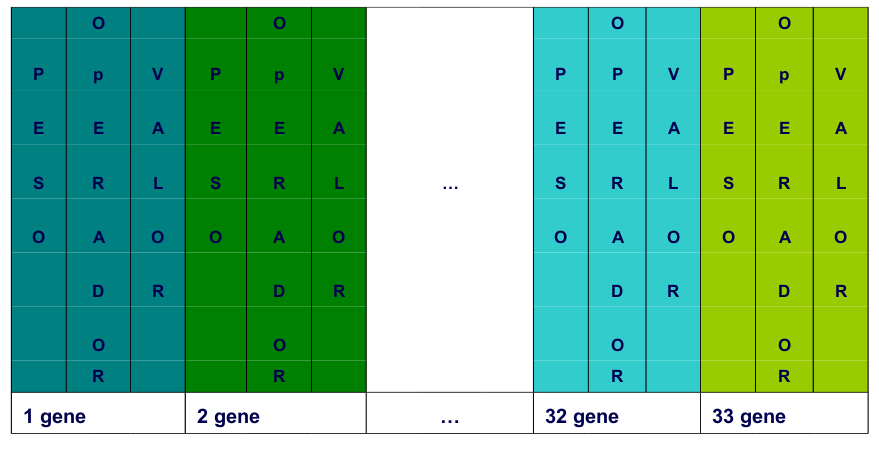
\includegraphics[width=8cm]{individuo.png}
  \caption{Representação de um indivíduo}
  \label{fig:individuo}
\end{figure}

Como parâmetros do algoritmo genético adotou-se uma população inicial de
50 individuos, taxa de cross over de 100\%, taxa de mutação de 30\%, número de
gerações igual a 50. A atualização da população é feita ordenando os pais e
filhos em ordem crescente de avaliação e pegando os 50 melhores, e configurou-se
como valor máximo de peso para o qual uma condição aparece sendo 0,3.

Para treinar o algoritmo e gerar as regras foi utilizado $2/3$ da base, em seguida
após as regras serem geradas as mesmas foram testadas utilizando o $1/3$ restante
dos dados.

\section{Contribuição do Trabalho}
\label{sec:contrib}

Contribuições da sua pesquisa sobre o tema abordado.

\section{Estado atual do Trabalho}
\label{sec:estado_atual}

Apresente a situação atual do andamento do desenvolvimento do trabalho. Caso haja necessidade, apresente detalhes sobre a metodologia para desenvolvimento do trabalho, incluindo materiais e métodos, descrição de ambiente e experimentos, etc. É facultada a apresentação do cronograma de desenvolvimento do trabalho.

\section{Análise de Resultados}
\label{sec:result}

Apresentação de resultados preliminares ou finais do trabalho de pesquisa.

\section{Trabalhos Relacionados}
\label{sec:trabalhos_relacionados}

Trabalhos relacionados, ilustrando a que ponto está o estado da arte junto à comunidade acadêmica, com pesquisas relacionadas à sua.

\bibliographystyle{sbc}
\bibliography{bib}

\end{document}
